\documentclass[10pt,a4paper]{article}
\usepackage[utf8]{inputenc}
\usepackage[spanish]{babel}
\usepackage{amsmath}
\usepackage{amsfonts}
\usepackage{amssymb}
\usepackage{makeidx}
\usepackage{graphicx}
\usepackage{lmodern}
\usepackage{kpfonts}
\usepackage{fourier}
\usepackage[hidelinks]{hyperref}
\usepackage[left=2cm,right=2cm,top=2cm,bottom=2cm]{geometry}
\author{Luis Angel Torres Pinto}
\title{Diseño de un Modulación de Ancho de Pulso (PWM) con Amp-OP y transistores.}
\begin{document}
\maketitle
\centering

\includegraphics[scale=2]{upzmg.jpg}\\
\newpage 
\raggedright
\section{¿Que es un PWM?}
Es un tipo de señal de voltaje utilizada para enviar información o para modificar la cantidad de energía que se envía a una carga. Este tipo de señales es muy utilizada en circuitos digitales que necesitan emular una señal analógica.
Este tipo de señales son de tipo cuadrada o sinusiodales en las cuales se les cambia el ancho relativo respecto al período de la misma, el resultado de este cambio es llamado ciclo de trabajo y sus unidades están representadas en términos de porcentaje. Matemáticamente se tiene que:\\
\centering
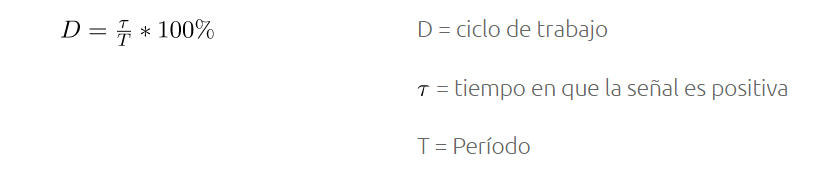
\includegraphics[scale=.70]{cal.png}\\ 
\raggedright
PWM son siglas en inglés que significan Pulse Width Modulation y que lo podemos traducir a español como Modulación de ancho de pulso. Puede ser que esto no te diga nada de momento, pero al terminar el artículo tomará todo el sentido del mundo.

La modulación de ancho de pulso está formada por una señal de onda cuadrada que no siempre tiene la misma relación entre el tiempo que esta en alto y el tiempo que está en bajo.

En la siguiente imagen vemos una señal que varía entre 5 voltios y 0 voltios. A lo largo del tiempo la señal varía entre dos valores de tensión. Durante un tiempo determinado la señal se encuentra en el nivel alto ( en este caso 5v ) y durante otro periodo de tiempo se encuentra en el segundo valor de tensión (en este caso 0v).\\
\centering
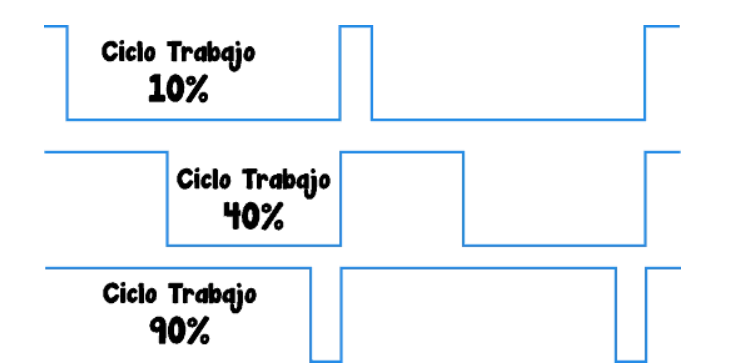
\includegraphics[scale=.80]{señ.png}\\
\raggedright
El tiempo que la señal se encuentra en el nivel alto ( 5 voltios ) lo denominamos como tiempo on ( Ton ) mientras que el tiempo que está en nivel bajo lo denominamos tiempo off ( Toff ). La suma del tiempo on y el tiempo off es el perido de la señal ( T ).

Y como en toda señal periódica, el inverso de del periodo ( 1 / T ) es la frecuencia de la señal.\\
\bigskip 
La construcción típica de un circuito PWM se lleva a cabo mediante un comparador con dos entradas y una salida. Una de las entradas se conecta a un oscilador de onda dientes de sierra, mientras que la otra queda disponible para la señal moduladora. En la salida la frecuencia es generalmente igual a la de la señal dientes de sierra, y el ciclo de trabajo está en función de la portadora.
La principal desventaja que presentan los circuitos PWM es la posibilidad de que haya interferencias generadas por radiofrecuencia. Éstas pueden minimizarse ubicando el controlador cerca de la carga y realizando un filtrado de la fuente de alimentación.

\section{¿Cómo funciona el PWM? }
Variando su valor de tensión entre dos valores conocidos, por ejemplo Vcc y GND en periodos concretos de tiempo y con una frecuencia fija. Estos periodos reciben nombres especiales.\\
\bigskip
Primero: Generador de ondas de dientes de sierra:\\
Hay muchas formas de generar este tipo de onda, utilizando compuertas, con un PIC, pero mi favorita es usando el histórico 555, y aun con este hay varias formas de generarla, una de ellas es utilizando el tiempo de carga y descarga del condensador que controla los tiempos del 555, pero como no aprendí muy bien esta forma, lo haré a mi manera, que es utilizando la salida del 555 para cargar y descargar otro condensador por medio de un transistor.
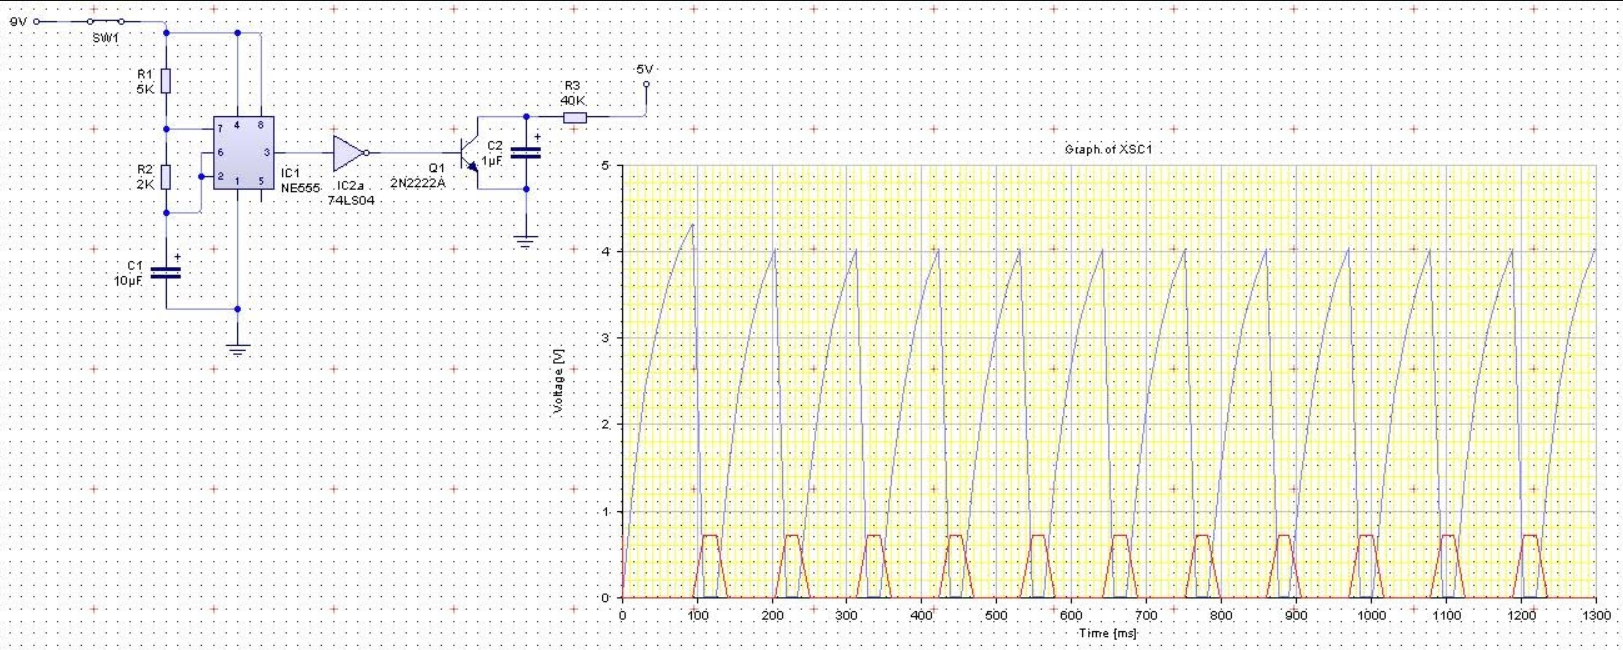
\includegraphics[scale=.42]{oon.png}\\
En este Diseño se compone de dos partes básicas, una el 555 configurado como astable con cierto periodo, donde el tiempo en alto es mayor al tiempo en bajo, tiempos que son invertidos gracias al inversor.\\
\bigskip
La segunda parte esta conformada por un condensador y un transistor, donde el transistor descarga por cada pulso al condensador generando así la onda con forma de dientes de sierra.\\ 
\bigskip
Segundo: Rampa (onda moduladora):\\
Es la parte mas sencilla de todo el diseño, se basa en el mismo concepto anterior de carga y descarga de un condensador, pero en este caso solo nos interesa la carga.\\
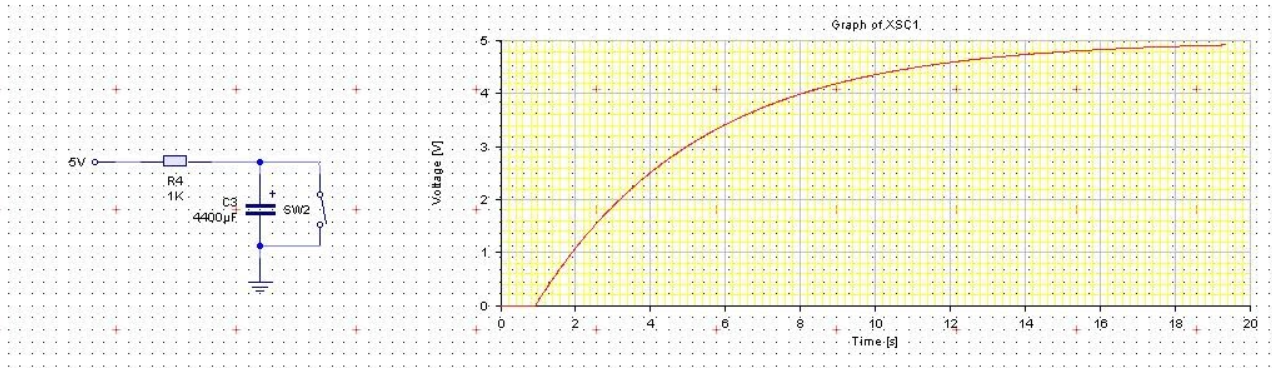
\includegraphics[scale=.55]{ond.png}\\
En este caso en vez de un transistor tenemos un switch, que por decirlo así es el encargado de poner en funcionamiento nuestro circuito, cuando esta cerrado el condensador esta descargado, no hay movimiento pero cuando se abre el condensador empieza a cargarse a determinada velocidad.\\
\bigskip
Tercero: Integración de los dos circuitos:\\
Ya teniendo los circuitos medianamente claros XD, nos preguntamos ¿y bueno eso para que? pues bueno una circuito de PWM consta de dos tipos de onda, una portadora(triangular o dientes de sierra) y una moduladora (la rampa), que se comparan atravez de un amplificador operacional y generan la PWM.
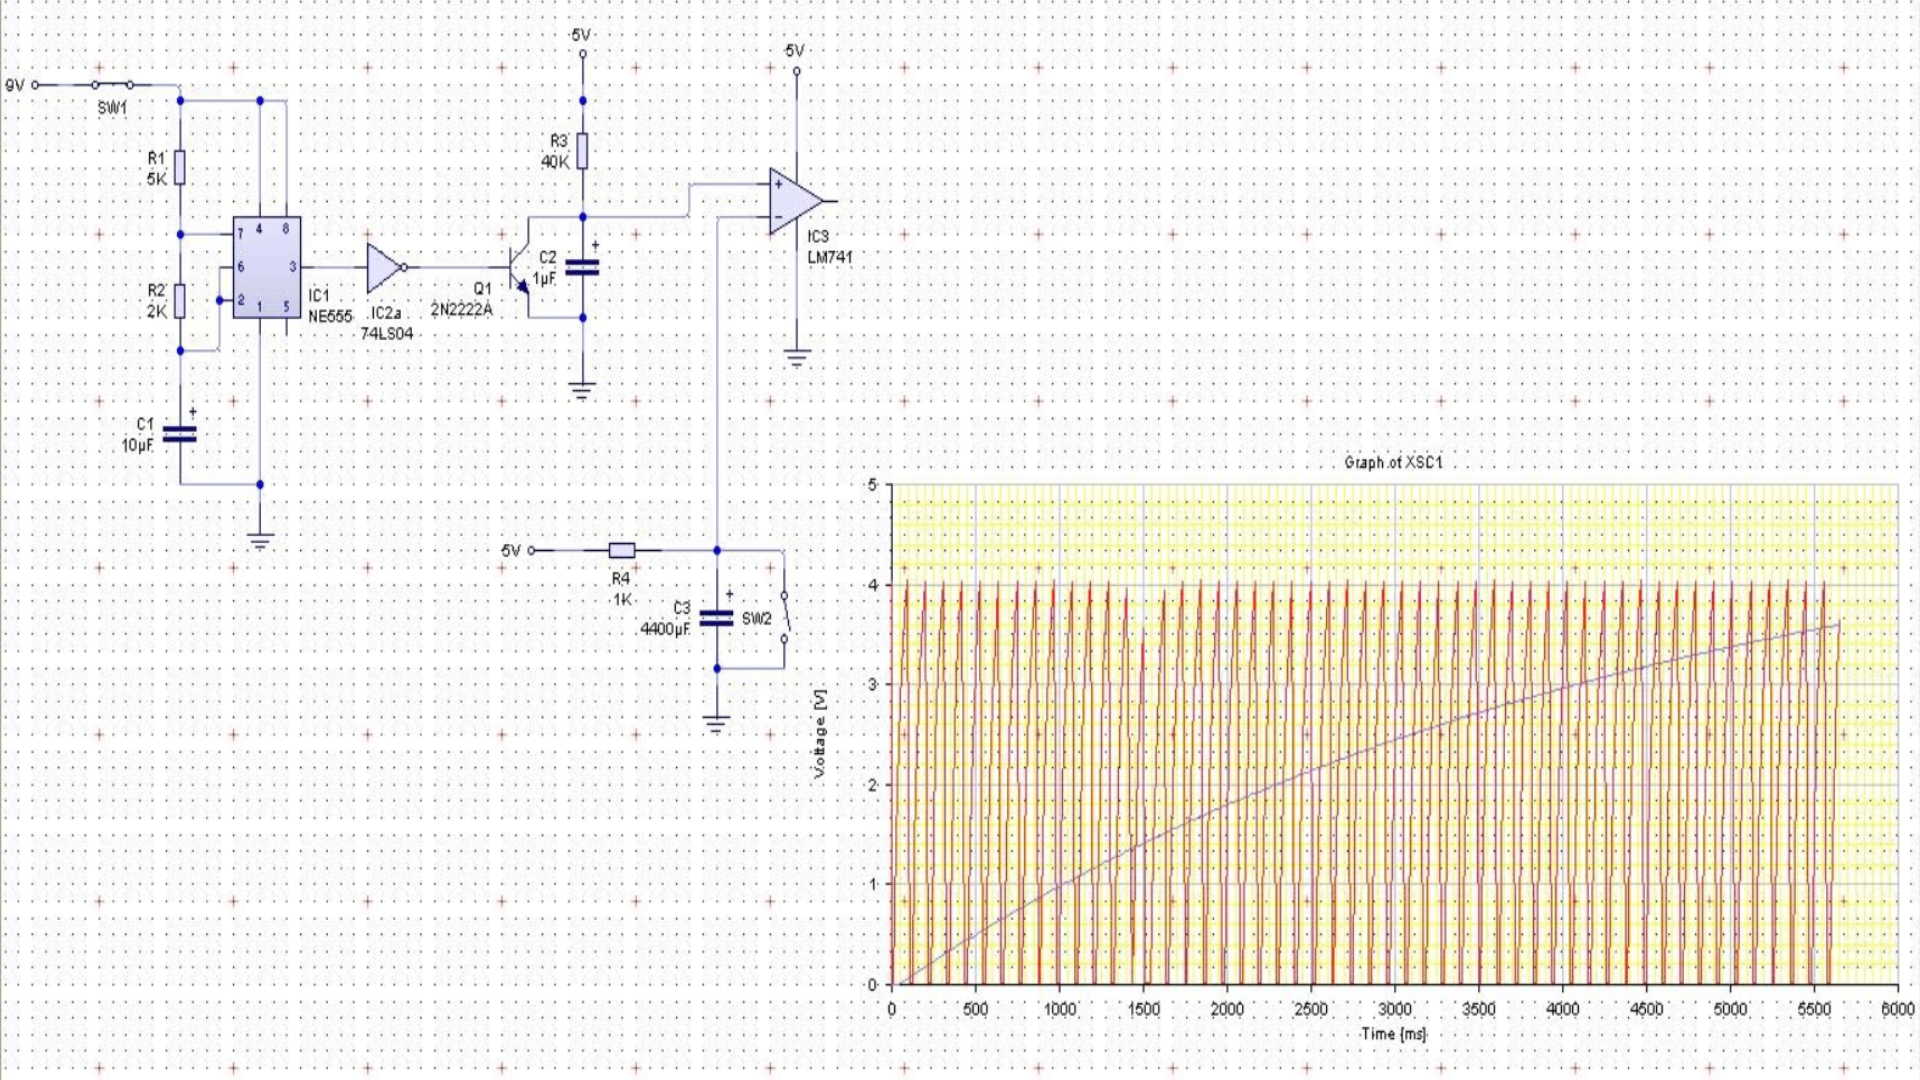
\includegraphics[scale=.35]{3.png}\\
\bigskip
Cuarto: Carga:\\
Ya lo único que falta es la carga, es decir lo que quieres controlar con este medio, en este caso les mostrare como poner un motor. el mecanismo es fácil, solo se trata de un transistor, para mejor uso un MOSFET, y la carga, el gate del MOSFET va conectada a la salida del amplificador operacional, el drain y el source son ya parte del otro circuito (a controlar).\\
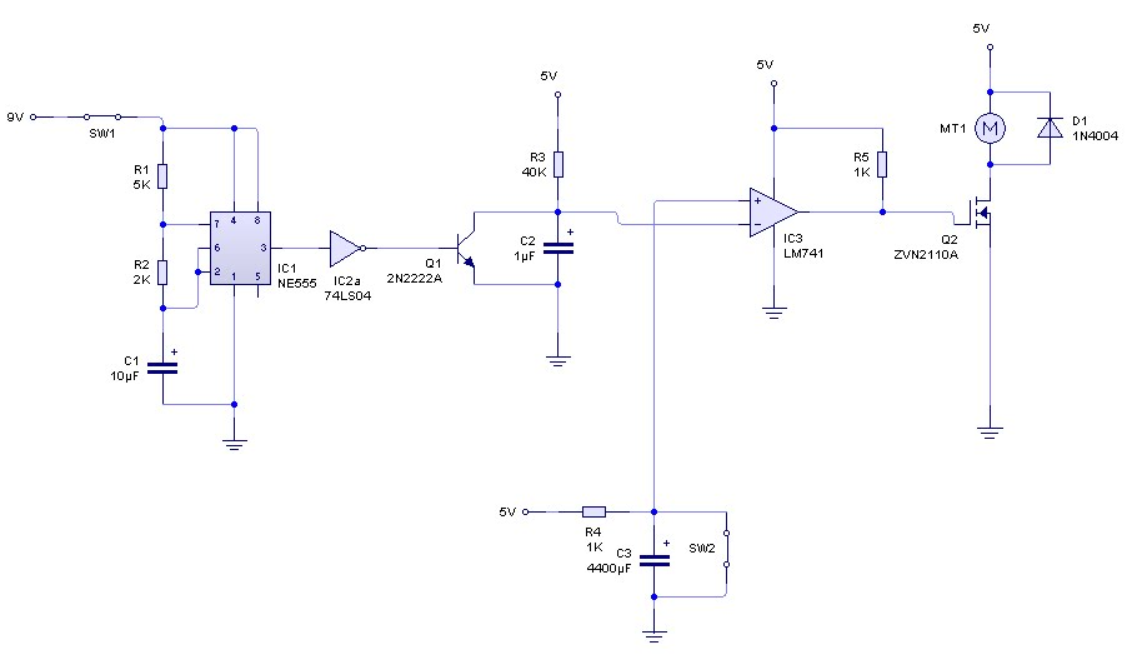
\includegraphics[scale=.50]{ul.png} \\
Así quedaria listo el diseño.\\
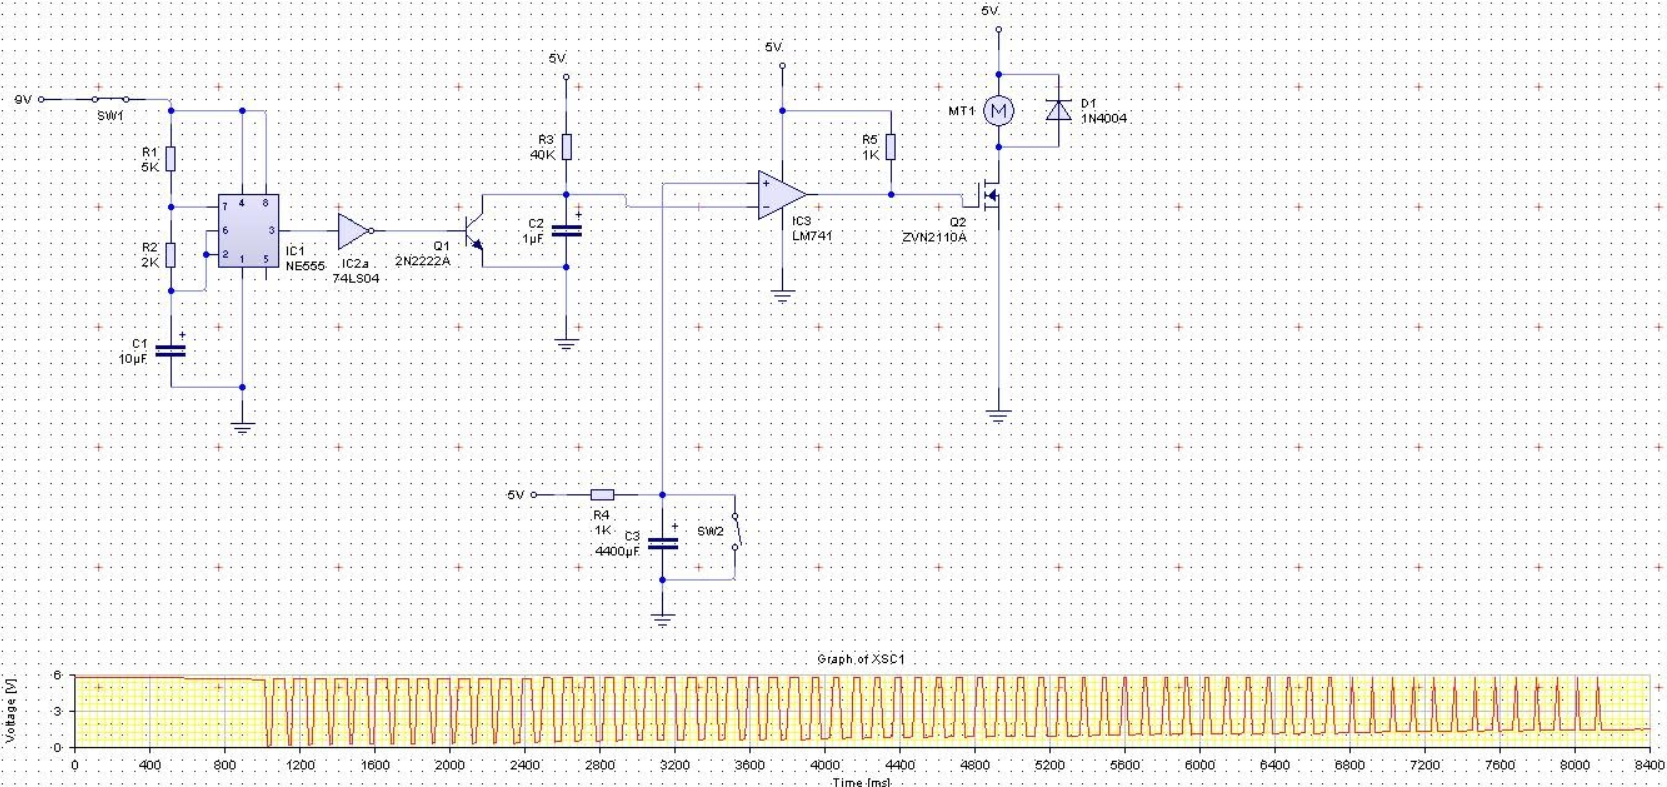
\includegraphics[scale=.40]{fin.png} 
\section{Materiales:}
IC1: 555\\
IC2: 74LS04\\
IC3: LM741\\

R1 5 Kohm\\
R2 2 Kohm\\
R3 40 Kohm\\
R4 y R5 1 Kohm\\

S1 y S2 Switchs On/Off\\

C1 10 uF Electrolitico\\
C2 1 uF Electrolitico\\
C3 4400 uF Electrolitico\\

Q1 2N2222A NPN\\
Q2 ZVN2110A o IRF640 MOSFET\\
\bigskip
Opcional:\\
MT1 Motor 6VC
D1 1N4004\\
\section{Referencias}
[1] Ram´on Pall´as Areny, Sensores y acondicionadores de se˜nal, Marcombo, Cuarta edic´on., 2003.\\
\bigskip
[2] Robert F. Coughlin, Frederick F. Driscoll, Amplificadores operacionales y circuitos integrados lineales.,Prentice Hall, 1993.\\
\bigskip
\url{https://www.rinconingenieril.es/que-es-pwm-y-para-que-sirve/}
\url{www.academia.edu/26259677/Modulador_de_Ancho_de_Pulso}

\end{document}